\chapter{Registers}

Each thread has access to a section of the register file, which is visible to the thread through the register specifiers in its instructions. This view of the register file is called the thread's \emph{logical} context, which is unrelated to the physical layout of the registers in the register file. The logical register context of a thread is separated into (up to four) different sections, each with different properties:

\begin{itemize}
\item Globals. The contents of these registers are provided by the parent thread of the family that the current thread belongs to. They contain read-only information which is independent from the index of the thread in the family and does not get modified during execution of the family. For instance, these registers can contain pointers to data structures, loop-invariants such a complex expressions, and so on.
\item Dependents. These registers map to the ``shared'' registers of the previous thread in the family's index sequence. See the next item for more details.
\item Shareds. These registers are available for reading by the next thread in the family's index sequence via its ``dependent'' registers. Combined, these two registers classes create a private, one-way communication channel between two adjacent threads in a family. Since such a channel exists between every adjacent pair of threads in the family, this creates a chain of possible efficient communication through the entire family without having to resort to memory for communicating small data between these threads.
\item Locals. These registers are available for private use to the current thread and that thread alone. No other thread is able to read or write these registers at any time.
\end{itemize}

\section{Virtual layout}
\label{sec:registers-virtual-layout}

\begin{figure}
 \begin{center}
  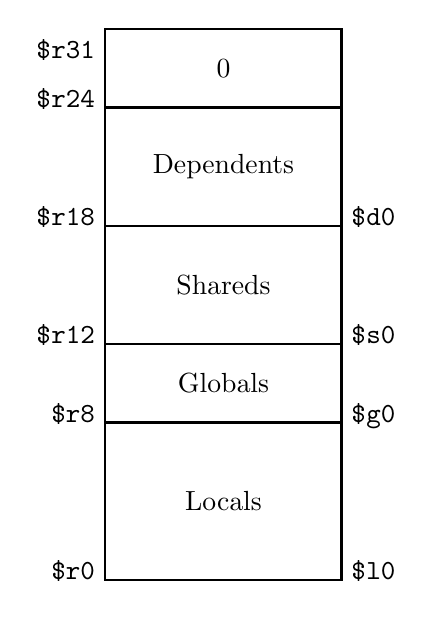
\begin{tikzpicture}[auto,thick,text badly centered]

	\begin{scope}[every node/.style={draw,rectangle,minimum width=3cm,outer sep=0cm}]
		\node[minimum height=2.0cm] (locals)                                   {Locals};
		\node[minimum height=1.0cm] (globals)    at (locals.north)     [above] {Globals};
		\node[minimum height=1.5cm] (shareds)    at (globals.north)    [above] {Shareds};
		\node[minimum height=1.5cm] (dependents) at (shareds.north)    [above] {Dependents};
		\node[minimum height=1.0cm] (zero)       at (dependents.north) [above] {0};
	\end{scope}
	
	\node at (locals.south west)     [above left, anchor=base east] {\tt \$r0};
	\node at (globals.south west)    [above left, anchor=base east] {\tt \$r8};
	\node at (shareds.south west)    [above left, anchor=base east] {\tt \$r12};
	\node at (dependents.south west) [above left, anchor=base east] {\tt \$r18};
	\node at (zero.south west)       [above left, anchor=base east] {\tt \$r24};
	\node at (zero.north west)       [below left] {\tt \$r31};
	
	\node at (locals.south east)     [above right, anchor=base west] {\tt \$l0};
	\node at (globals.south east)    [above right, anchor=base west] {\tt \$g0};
	\node at (shareds.south east)    [above right, anchor=base west] {\tt \$s0};
	\node at (dependents.south east) [above right, anchor=base west] {\tt \$d0};
	
\end{tikzpicture}
  \caption{Virtual layout of a thread's integer registers with 8 locals, 4 globals and 6 shareds and dependents. On the left are the base ISA's register specifier. On the right are their alternative specifiers which indicate the sections. Note that only 24 of the 32 registers are used; {\tt \$r24}--{\tt \$r31} are read-as-zero. In this example the base ISA is from the DEC Alpha.}
  \label{fig:regs-virtual}
 \end{center}
\end{figure}

The compiler determines the size of these four regions (with the shareds and dependents equally sized) based on the thread code, with the constraint that all these sections must fit in the original ISA's register context\footnote{For instance, on a traditional RISC architecture with 5-bit register specifiers with a single read-as-zero register, the sum of the sizes of these sections cannot exceed 31.}. As a result, the compiler simply uses these section by using the correct register specifier from the base ISA. Figure~\ref{fig:regs-virtual} shows this mapping. Note that any or all of these sections can be of zero size. 

\section{Physical layout}

\begin{figure}
 \begin{center}
  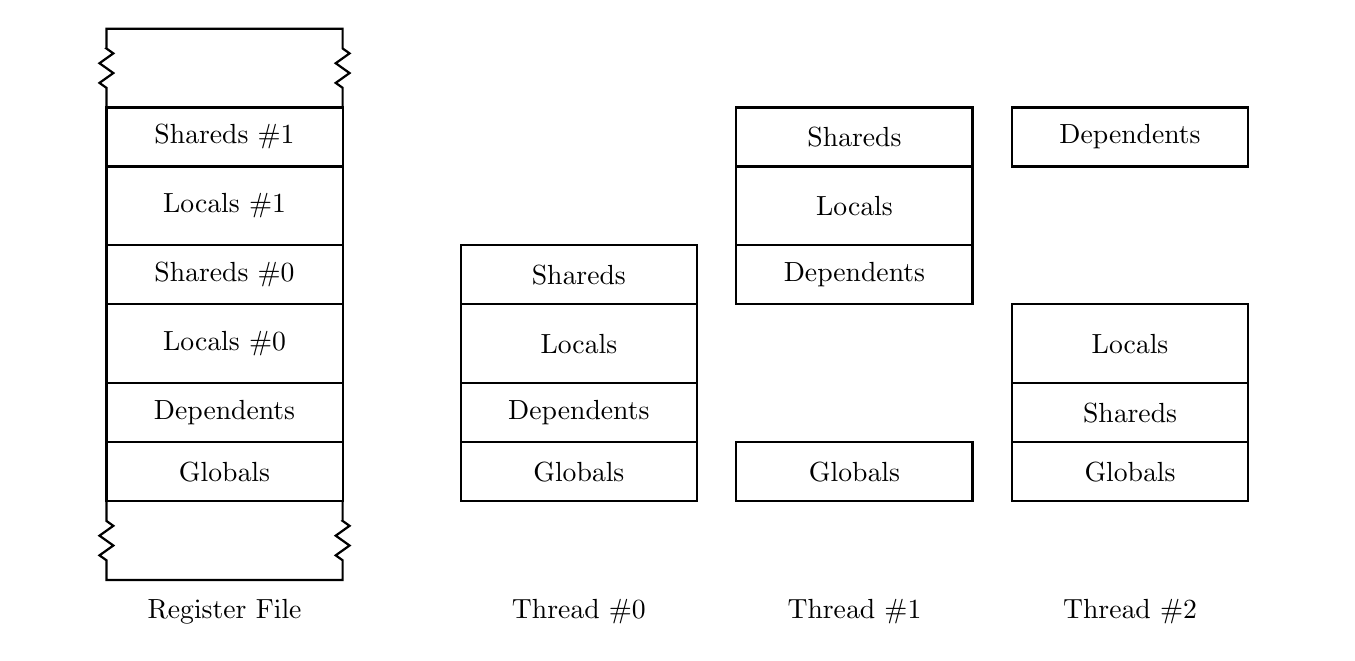
\begin{tikzpicture}[auto,thick,text badly centered,every node/.style={outer sep=0cm}]

	\begin{scope}[every node/.style={draw, rectangle, minimum width=3cm, outer sep=0cm}]
		\node[minimum height=0.75cm] (g)                     	{Globals};
		\node[minimum height=0.75cm] (d)  at (g.north)  [above] {Dependents};
		\node[minimum height=1.00cm] (l0) at (d.north)  [above] {Locals \#0};
		\node[minimum height=0.75cm] (s0) at (l0.north) [above] {Shareds \#0};
		\node[minimum height=1.00cm] (l1) at (s0.north) [above] {Locals \#1};
		\node[minimum height=0.75cm] (s1) at (l1.north) [above] {Shareds \#1};
	\end{scope}
	
	\begin{scope}[decoration={zigzag, segment length=0.25cm}]
		\draw (g.south west)  -- +(0,-0.25) decorate {-- +(0,-0.75)} |- +(3,-1.0) -- +(3,-0.75) decorate {-- +(3,-0.25)} -- (g.south east);
		\draw (s1.north west) -- +(0, 0.25) decorate {-- +(0, 0.75)} |- +(3, 1.0) -- +(3, 0.75) decorate {-- +(3, 0.25)} -- (s1.north east);
	\end{scope}
	
	\node[minimum width=5cm] (rf) at (g)  [below=1.5cm] {Register File};
	\node[minimum width=5cm] (t0) at (rf) [right=2cm] {Thread \#0};
	\node[minimum width=5cm] (t1) at (t0) [right=1cm] {Thread \#1};
	\node[minimum width=5cm] (t2) at (t1) [right=1cm] {Thread \#2};
	
	\begin{scope}[every node/.style={draw, rectangle, minimum width=3cm, outer sep=0cm}]
		\node[minimum height=1.00cm] (t0_l) at (l0 -| t0) {Locals};
		\node[minimum height=1.00cm] (t1_l) at (l1 -| t1) {Locals};
		\node[minimum height=1.00cm] (t2_l) at (l0 -| t2) {Locals};
	
		\node[minimum height=0.75cm] (t0_s) at (s0 -| t0) {Shareds};
		\node[minimum height=0.75cm] (t1_s) at (s1 -| t1) {Shareds};
		\node[minimum height=0.75cm] (t2_s) at (d  -| t2) {Shareds};
	
		\node[minimum height=0.75cm] (t0_d) at (d  -| t0) {Dependents};
		\node[minimum height=0.75cm] (t1_d) at (s0 -| t1) {Dependents};
		\node[minimum height=0.75cm] (t2_d) at (s1 -| t2) {Dependents};
	
		\node[minimum height=0.75cm] (t0_g) at (g -| t0) {Globals};
		\node[minimum height=0.75cm] (t1_g) at (g -| t1) {Globals};
		\node[minimum height=0.75cm] (t2_g) at (g -| t2) {Globals};
	\end{scope}
	
\end{tikzpicture}
  \caption{Phsyical and virtual layout of the integer registers of a family's threads. On the left is the physical register file with allocated registers. On the right are the first three threads in the family and their virtual register sections.}
  \label{fig:regs-physical}
 \end{center}
\end{figure}

The virtual registers as described in the previous section are mapped onto the core's physical register file. This register file contains the contexts of many threads. During the family creation process on a core, a section of contiguous registers are allocated to accomodate $N$ threads (see section~\ref{sec:register-alloc} for details and how $N$ is chosen). This single block of registers is divided among the threads of that family on that core. However, this division is non-trivial. Trivially, by their nature, the global registers for every thread are mapped onto the same physical registers. Mapping the local registers is similary trivial, where a simple offset can be used to obtain a thread's private space in the block of allocated registers.

However, if the family's threads contain shareds and dependents, the dependents of thread $i+1$ have to be mapped to the shareds of thread $i$, with exceptions for the first and last thread in the family. The dependents of the first thread in a family have no shareds to be mapped onto, so they have their own section of registers. The parent thread can then fill these registers with a special register-move instruction; this mechanism is used to initialize the shareds-dependents chain through the family. Similarly, the shareds of last thread in a family have no dependents mapped onto them. Instead, the parent thread uses a register-move instruction to copy their contents back to its own context, thus retrieving the ``output'' value of the shareds-dependents chain.

Since threads in a family are allocated in-order, the shareds-dependents chain can be constructed by mainting a ``last allocated'' pointer in the family table that points to the shareds of the last allocated thread of that family. Coupled with this, every thread has a pointer in the thread table that points to its dependents, which the pipeline can use to decode the virtual register specifier into a physical register specifier. In this case, thread creation involves copying the ``last allocated'' pointer from the family table to the newly created thread's dependent pointer and setting the ``last allocated'' pointer to this thread's shareds.

Figure~\ref{fig:regs-physical} shows an example of this mapping of the virtual contexts of threads in a family onto the physical register file.

Note that the shareds of threads 2 overlap with the dependents of thread 0. One might assume that if thread 2 writes to its shareds, it will overwrite the dependents of thread 0. However, because there's only enough space in the allocated registers for two threads, at most two threads will exist at any time. As a result, if thread 2 exists, thread 0 must have terminated, freeing its locals and dependents for reuse.

\subsection{\label{sec:registers-family-creation}Family Creation}
When a family is created (see section~\ref{sec:family-setup}), the program can optionally specify a \emph{block size}. This specifies a distribution size for a group family across multiple cores \emph{and} an upper limit on the number of threads allocated at any time to this family, per core. The latter meaning of this value is of relevance to the allocation of registers. During family creation, the core attempts to allocate this many thread's worth of registers. If this cannot succeed, fewer and fewer threads worth of register will try to be allocated until a block of registers can be allocated which can accomodate $N$ registers. This value is known as the \emph{physical} block size, whereas the originally specified value is the \emph{virtual} block size. The physical block size now determines how many threads can, at most, be allocated on this core.

After the core has finished allocating resources, including its register block, for the family, the family is moved to the \emph{thread allocation list}, where another process will start allocating threads from it.

\subsection{Thread Creation}
A process on each core is responsible for taking allocated families and allocating threads to that family until the number of threads allocated to that family equals the family's physical block size (see section~\ref{sec:thread-alloc}). However, to avoid complicated allocation logic, when a thread can be cleaned up and its family still has threads in its index sequence that have not yet been creeated, the thread's entry is reused for the next thread in the family. This operation is performed by the same process. Thus, this process has two inputs: the family at the head of the thread allocation list, and the thread cleanup queue. The thread creation process is responsible for setting up the pointers in the thread table to the register file where the thread's locals, dependents and shareds are located (the address to the globals is thread independent and are stored in the family table). But, this operation dependents on whether the new thread uses a new entry, or reuses an old one.

When a new thread is created at an unused thread table entry, its register addresses must be initialized. The family maintains a counter, {\tt thread\_count}, which indicates how many physical threads have been allocated to this family. This counter starts at zero, is incremented with every newly allocated thread and will never be more than the number of allocated register contexts. This counter can be used to find the next context in the allocated registers which is still untouched. This context's offset is determined by skipping the base globals and dependents and {\tt thread\_count} worth of contexts (locals and shareds), which have already been allocated to existing threads. The new thread's shareds lie in this block as well, above the locals. 

When a thread entry is reused for a new thread, the new thread can reuse the old thread's locals for its own. The only offsets that need to change are for the thread's dependents and shareds. The old thread's dependents are no longer in use and can be reused for the new thread's shareds, a simple copy from one field in the thread table to the other. The new thread's dependents are the last allocated thread's shareds.

Note in both cases, the new thread's dependents are the last allocated thread's shareds, which involves a simple copy from one field in the family table to the thread table.